\documentclass[%
 aps, reprint, prl, amsmath,amssymb
]{revtex4-2}

\usepackage{graphicx}% Include figure files
\graphicspath{{figures/}} 
\usepackage{dcolumn}% Align table columns on decimal point
\usepackage{bm}% bold math
\usepackage{orcidlink}
\usepackage{mathtools}
\usepackage{algpseudocode}

% -------------- Watermark ----------------
\usepackage[style=iso]{datetime2}
\usepackage{FiraMono} 
\usepackage{tikz}
\usepackage{transparent} 

% Use shipout/background to ensure it stays behind text/figures
\AddToHook{shipout/background}{
  \begin{tikzpicture}[remember picture, overlay]
    \node [
      rotate=55,
      scale=1.2,
      text opacity=0.15,      
      color=gray!50,          
      font=\fontfamily{FiraMono-TLF}\selectfont\bfseries,
      align=center
    ] at (current page.center) {
        {\fontsize{60}{70}\selectfont WORKING DRAFT} \\ [0.8cm]
        {\Huge \DTMnow} \\
        {\Huge doi.org/10.17605/OSF.IO/EV8H6} \\ [0.8cm]
        {\Large Computational Complex Systems Laboratory} \\
        {\Large Homey Music, Detroit, USA} \\ [0.2cm]
         {\transparent{0.25}\includegraphics[width=1.0cm]{logo.png}}
    };
  \end{tikzpicture}
}
% -----------------------------------------


\DeclareMathOperator*{\argmin}{argmin}
\begin{document}

\title{Information Erasure Inside the Quantum of Action}

\begin{abstract}
Quantum microstates are operationally indistinguishable inside Planck's quantum of action. We show that Landauer's principle compels the erasure of each microstate into the minimal-action state. This erasure coarse-grains the classical continuum, selecting the discrete configurations of quantum mechanics.
\end{abstract}


\author{Brian S. Mulloy\orcidlink{0000-0002-1803-3172}}
\email{brian@homeymusic.com}
\affiliation{Computational Complex Systems Laboratory\\Homey Music, Corktown, Detroit, MI, USA}
\date{\today}

\maketitle
\subsection{Erasure Action}

\begin{equation}
\label{eq:SimpleLanguageHero}
\text{Erasure Action} \le \text{Classical Action}
\end{equation}

\begin{equation}
\label{eq:Hero}
K E_L \tau \le A
\end{equation}

\subsection{The Quantum Blob}

\begin{equation}
\label{eq:HeisenbergVariance}
\sigma_q \sigma_p \ge \frac{\hbar}{2}
\end{equation}

\begin{equation}
\label{eq:CovarianceEllipsoid}
\frac{q^2}{2\sigma_q^2} + \frac{p^2}{2\sigma_p^2} \le 1
\end{equation}

\begin{equation}
\label{eq:EllipsoidArea}
A = \pi (\sqrt{2}\sigma_q) (\sqrt{2}\sigma_p) = 2\pi \sigma_q \sigma_p
\end{equation}

Saturating the Heisenberg bound ($\sigma_q \sigma_p = \hbar/2$) gives the minimum area:

\begin{equation}
\label{eq:SymplecticCapacity}
A_{\text{blob}} = 2\pi \left( \frac{\hbar}{2} \right) = \frac{h}{2}
\end{equation}

De Gosson \cite{DeGosson2009Iceberg} recalled the symplectic camel to characterize this invariant topological capacity:

\begin{quote}
``It is easier for a camel to pass through the eye of a needle than for one who is rich to enter the kingdom of God.'' \cite{NABRE2011}
\end{quote}

\begin{figure}[t!]
    \centering
    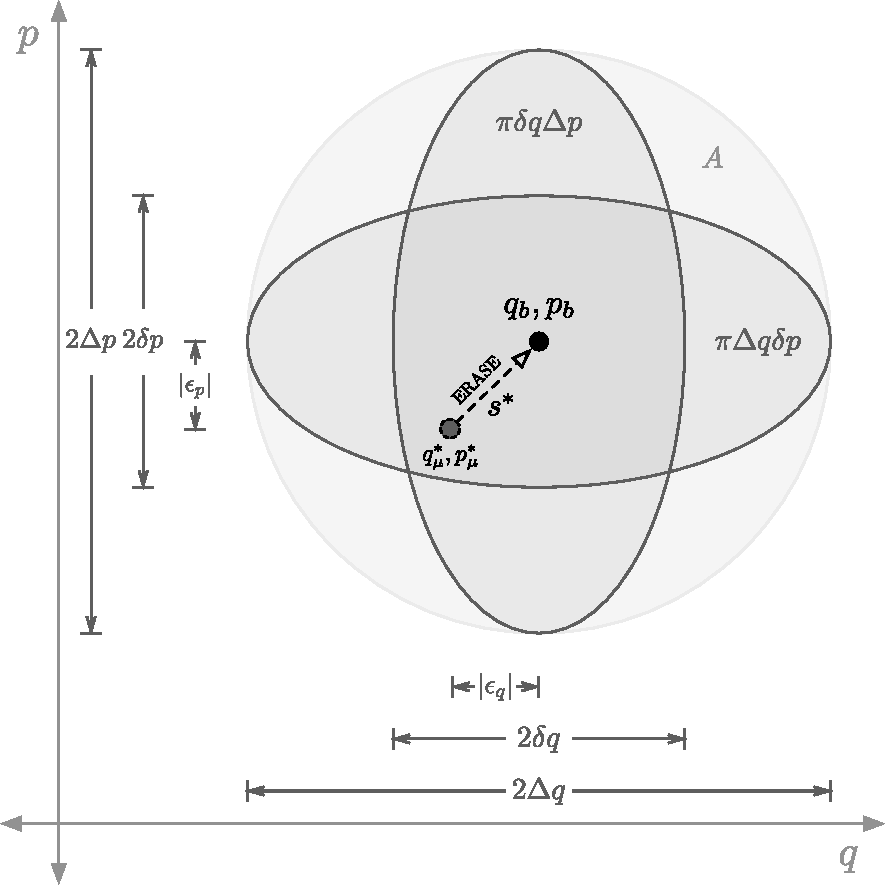
\includegraphics[width=\linewidth]{erase.pdf}
\caption{\textbf{Information erasure inside the quantum of action} (schematic). Boundaries $\Delta q$ and $\Delta p$ determine the classical action area $A$ in phase space. The reciprocal relations $\delta q = \hbar / \Delta p$ and $\delta p = \hbar / \Delta q$ characterize the symplectic squeezing of the conjugate pair of quantum blobs, $\pi \delta q \Delta p = \frac{h}{2}$ and $\pi \Delta q \delta p = \frac{h}{2}$, whose sum is the quantum of action $h$. The values $\epsilon_q$ and $\epsilon_p$ are the erasure distances from each microstate $(q_\mu, p_\mu)$ with binary encoding $s_\mu$ to the minimal-action state $(q^*,p^*)$ with the minimal binary encoding $s^*$, where the minimal bit count is the Kolmogorov complexity $K = |s^*| \le |s_\mu|$. The physical scales satisfy $|\epsilon_q| \le \delta q \le \Delta q$ and $|\epsilon_p| \le \delta p \le \Delta p$.}
\label{fig:erase_schematic}
\end{figure}

\subsection{One Blob or Two?}

Zurek \cite{Zurek2001} demonstrated that a quantum state constrained by the classical action boundaries $\Delta q$ and $\Delta p$ develops sub-Planck structures defined by the reciprocal limits:

\begin{equation}
\label{eq:BlobSqueeze}
\delta q = \frac{\hbar}{\Delta p} \quad \text{and} \quad \delta p = \frac{\hbar}{\Delta q}
\end{equation}

Expressing Zurek's reciprocal limits as phase-space areas yields a conjugate pair of de Gosson capacities (see Fig.~\ref{fig:erase_schematic}):

\begin{equation}
\label{eq:BlobAreas}
\pi \delta q \Delta p = \frac{h}{2} \quad \text{and} \quad \pi \Delta q \delta p = \frac{h}{2}
\end{equation}

Because both areas are required to bound the space, the total quantum of action $h$ is defined by their geometric sum:

\begin{equation}
\label{eq:SimpleLanguageBlobs}
\text{Quantum of Action} = \text{Pair of Quantum Blobs}
\end{equation}

\begin{equation}
\label{eq:Blobs}
h = \pi \delta q \Delta p + \pi \Delta q \delta p
\end{equation}

This pair of quantum blobs with reciprocal proportionality evokes the \textit{r\'{i}astrad} of the Old Irish hero C\'{u} Chulainn:

\begin{quote}
``He squeezed one eye no wider than the eye of a needle; he opened the other wider than the mouth of a mead-cup.'' \cite{RiastradNote}
\end{quote}


\subsection{Quantum Density from Erasure}

In standard phase-space formulations, the density of states is modeled statistically using the continuous Wigner quasi-probability distribution $W(q,p)$. Here, the observed density is the deterministic result of the Landauer erasure distribution $L(q,p)$.

When the environment erases a continuous microstate $(q_\mu, p_\mu)$ into the minimal-action state $(q^*, p^*)$, the physical erasure distances are bounded by the classical action and the reciprocal sub-Planck structures: $\epsilon_q = q_\mu - q^*$ and $\epsilon_p = p_\mu - p^*$, such that $|\epsilon_q| \le \delta q \le \Delta q$ and $|\epsilon_p| \le \delta p \le \Delta p$. The observed coordinates are directly proportional to this thermodynamic displacement:

\begin{equation}
\label{eq:ObservedCoordinates}
q = \frac{A}{h} \epsilon_q \quad \text{and} \quad p = \frac{A}{h} \epsilon_p
\end{equation}

Let $N$ be the total ensemble of observed microstates. The Landauer erasure distribution $L(q,p)$ counts the exact number of microstates deterministically erased into each observed phase-space coordinate via the indicator function $\mathbb{I}$:

\begin{equation}
\label{eq:JointErasure}
L(q,p) = \sum_{\mu=1}^{N} \mathbb{I}\left( \frac{A}{h} \epsilon_q = q \right) \mathbb{I}\left( \frac{A}{h} \epsilon_p = p \right)
\end{equation}

In standard phase-space mechanics, the observable marginal densities are obtained by integrating the Wigner function over the conjugate variable. In our deterministic framework, the discrete state counts $N(q)$ and $N(p)$ emerge naturally by summing the Landauer erasure distribution $L(q,p)$ over the conjugate observables:

\begin{equation}
\label{eq:MarginalQ}
N(q) = \sum_{p} L(q,p)
\end{equation}

\begin{equation}
\label{eq:MarginalP}
N(p) = \sum_{q} L(q,p)
\end{equation}

These discrete marginals recover the physical structure of the expected quantum densities strictly through the thermodynamic coarse-graining of the classical continuum (see Fig.~\ref{fig:harmonic_oscillator}).



\subsection{The Relationship Between Bits and Resolving Power}

\begin{equation}
\label{eq:ResolvingPowerPlain}
\text{Resolving Power} \propto \text{Bits} \propto \text{Conjugate}
\end{equation}

\begin{equation}
\label{eq:ResolvingPower}
\mathcal{R}_q = \frac{1}{\delta q}  \quad \text{and} \quad \mathcal{R}_p = \frac{1}{\delta p}
\end{equation}

\begin{equation}
\label{eq:BitBudgetResolution}
\mathcal{R}_q \propto K_q \propto \Delta p \quad \text{and} \quad \mathcal{R}_p \propto K_p \propto \Delta q
\end{equation}

\subsection{Zurek Uncertainty Principle}

\begin{equation}
\label{eq:GeometricUncertaintyPrinciplePlainLanguage}
\text{Uncertainty} \propto \frac{1}{\text{Classical Action}}
\end{equation}

\begin{equation}
\label{eq:ZurekUncertaintyPrinciple}
\delta q \delta p = \frac{\hbar^2}{\Delta q \Delta p}
\end{equation}

\begin{figure}[t!]
    \centering
    \includegraphics[width=\linewidth]{figures/john_ellipse.pdf}
\caption{\textbf{The John Ellipse Uncertainty} (schematic). The area of the John ellipse contained within the orthogonal pair of quantum blobs is $\pi \delta q \delta p = \frac{h^2}{4 \pi \Delta q \Delta p}$, which yields the uncertainty relation $\delta q \delta p = \frac{\hbar^2}{\Delta q \Delta p}$.}
\end{figure}


\subsection{Excess Action}

\begin{equation}
\label{eq:ExcessAction}
\xi_q = \delta q - |\epsilon_q| \quad \text{and} \quad \xi_p = \delta p - |\epsilon_p| 
\end{equation}

\section{Correspondences}

\begin{itemize}
    \item characteristic time and quantum speed limits $\tau_{K=2}=\tau_\perp = \frac{h}{4 E_L}$
    \item erasure temperatures $T$ 
    \item information flux and van der Pauw $\frac{\pi}{\ln{2}}$
    \item Bekenstein bounds
    \item Fisher information
    \item Zurek tile $a$ and uncertainty
    \item Susskind's ``Complexity equals Action''
\end{itemize}

\section{Dimensionless Equations}

\begin{align}
\pi \delta q \Delta p &= \frac{h}{2} \\
\delta q &= q_0 \widetilde{\delta q} \\
\Delta p &= p_0 \widetilde{\Delta p} \\
\pi q_0 p_0 &= \frac{h}{2} \\
\pi q_0 p_0 \widetilde{\delta q} \widetilde{\Delta p} &= \frac{h}{2} \\
\widetilde{\delta q} \widetilde{\Delta p} &= 1 \\
\widetilde{\delta q} &= \frac{1}{\widetilde{\Delta p}}
\end{align}

\section{Numerical Simulations}

Let the generic variable $x \in \{q, p\}$ denote any phase-space component.

\begin{algorithmic}[1]
\Function{erase}{$x_\mu, \delta x$}
    \State $\text{left} \gets (-1, 0)$
    \State $\text{num} \gets 0, \quad \text{den} \gets 1$
    \State $\text{right} \gets (1, 0)$
    \State $x^* \gets \text{num} / \text{den}$
    \State $\mathbf{s}^* \gets \text{""}$
    \While{$|x_\mu - x^*| > \delta x$}
        \If{$x^* < x_\mu$} 
            \State $\text{left} \gets (\text{num}, \text{den})$
            \State $\mathbf{s}^* \gets \mathbf{s}^* + \text{'1'}$
        \Else 
            \State $\text{right} \gets (\text{num}, \text{den})$
            \State $\mathbf{s}^* \gets \mathbf{s}^* + \text{'0'}$
        \EndIf
        \State $\text{num} \gets \text{left}_{num} + \text{right}_{num}$
        \State $\text{den} \gets \text{left}_{den} + \text{right}_{den}$
        \State $x^* \gets \text{num} / \text{den}$
    \EndWhile
    \State $\epsilon_x \gets x^* - x_\mu$
    \State \Return $\epsilon_x, x^*, \mathbf{s}^*$
\EndFunction
\end{algorithmic}

\subsection{The Harmonic Oscillator Simulation}

\section{Foundational Manuscripts}

\begin{itemize}
    \item \textbf{Uncertainty}
    \begin{itemize}
        \item Heisenberg \cite{Heisenberg1927}
        \item de Gosson \cite{DeGosson2003}
        \item Zurek \cite{Zurek2001}
    \end{itemize}
    
    \item \textbf{Thermodynamics}
    \begin{itemize}
        \item Landauer \cite{Landauer1961}
        \item Margolus and Levitin \cite{MargolusLevitin1998}
    \end{itemize}
    
    \item \textbf{Stern-Brocot Tree}
    \begin{itemize}
        \item Graham, Knuth, and Patashnik \cite{ConcreteMath}
        \item Aiylam \cite{Aiylam2013}
    \end{itemize}
    
    \item \textbf{Criticism of Macroscopic $\Delta q \Delta p$}
    \begin{itemize}
        \item Schr\"{o}dinger \cite{Schrodinger1980Trimmer}
    \end{itemize}

\end{itemize}

\bibliography{main} 
\end{document}
